\documentclass[12pt,a4paper]{article}
\usepackage[dutch]{babel}
\usepackage{graphicx}

\author{Wannes Sergeant}
\title{Testbestand Wannes Sergeant}
\date{\today}

\begin{document}
    \maketitle
    
\section{Dit is een titel}
\label{sec:intro}

\subsection{Dit is nog iets}
    
    Dit is een referentie naar hoofdstuk \ref{sec:intro}
    
    \begin{enumerate}
        \item bla
        \item blabla
        \item blablabla
    \end{enumerate}

    % Dit is een figuur
    \begin{figure}
        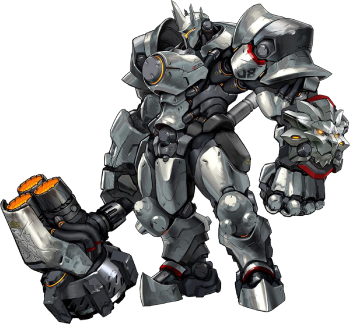
\includegraphics[width=0.7\textwidth]{img/reinhardt.jpg}
        \caption{Dit is Reinhardt. Reinhardt is machtig!}
        \label{fig:reinhardt}
    \end{figure}

    Dit is een figuur van Reinhardt en die vind je in figuur \ref{fig:reinhardt}
    
\end{document}